Při použití tlustovrstvé technologie je potřeba uvědomit si faktory, které ovlivňují výslednou kvalitu a spolehlivost. Těchto faktorů je mnoho a odvíjí se zejména od použité technologie. 
  Např. při sítotisku musíme vzít v potaz parametry zvolené pasty, substrátu, na který nanášíme, a v neposlední řadě také samotného síta. Optimálního výsledku dosáhneme pouze vhodnou kombinací všech zmíněných faktorů. 

  Dnešní práce se věnuje vlastnotem používaných past. 
  
  \subsection{Reologické vlastnosti}
  Reologie je nauka o tomu a plynutí materiálů. Pro obecný popis tekutosti materiálu můžeme využít tzv. Debořino číslo T:
  \[
    T=  \frac{T_{rel}}{T_{obs} }
  \]
  kde \(T_{rel} \) je relaxační doba daného materiálu a \(T_{obs} \) je doba pozorování.
	
  \subsubsection{Viskozita}
    Viskozita popisuje vnitřní tření kapalin, to ovšem není konstantní, naopak je závislé na několika faktorech, např. na teplotě, složení a koncentraci roztoku a tlaku. 
    Obvykle pracujeme s pojmem \textbf{Dynamická viskozita}, jedná se o fyzikální veličinu značenou \(\eta\), udává odpor, který kladou dvě sousední vrstvy kapaliny vzájemnému pohybu. 
    Jednotkou viskozity je poise (P), ten je definován následovně:
    \[
      \qty{1}{P} = \qty{1}{\gram\per\centi\meter\per\second}
    \]
    \[  
        \qty{10}{P} = \qty{1}{\pascal\second}
    \]
    Převrácenou hodnotou viskozity je \textbf{fluidita} neboli tekutost. 

    \begin{figure}[h!]
      \centering
      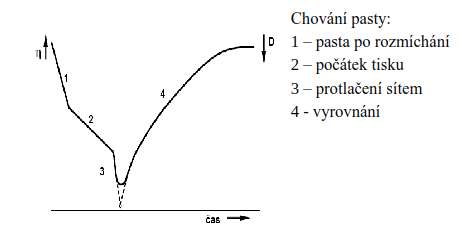
\includegraphics[width=0.6\textwidth]{viskozita.png}
      \caption{Časová závislost viskozity při nanášení pasty těrkou, mění se tedy tlak.}
      \label{fig:viskozita-png}
    \end{figure}
    

    \subsection{Zrnitost}
      Pasty používané v tlustovrstvé technologii se ovykle skládají ze tří hlavních složek, funkční, tavivové a pojivové \cite{DiplomkaTlusteVrstvy}. Funkční složka je obvykle tvořena pevným práškem žádaného materiálu a společně s částicemi tavivové složky, která po výpalu tuhne a tvoří tvar výsledné vrstvy jsou rozptýleny v pojivu, to určuje zejména viskozitu pasty při jejím zpracování. Při práci s pastou musíme vzít v potaz velikost zrn ve funkční a tavivové složce. Ta by měla být pokud možno co nejvíce definovaná, stejně tak i tvar zrn. 
      Obvykle se pohybujeme v hodnotách od 1 do \qty{10}{\micro\meter} \cite{zadani}. Velikost zrn určuje mimo jiné také minimální tloušťku nátěru. 
      
      Určení velikosti zrn je možné za pomoci \textbf{grindometru}\cite{zadani}. Princip měření spočívá v rozetření pasty přes nakloněnou rovinu při konstantní výšce stěrky. V určitém bodě už zrna nevejdou do prostoru mezi rovinu a stěrku a jsou tedy setřeny pryč. Přístroj obsahuje stupnici, kde je možné následně odečíst požadovanou hodnotu velikosti zrn. 
	
    \subsection{Adheze}
      \subsubsection{Scratch test}
      Jednou z metod pro testování adheze tlustých vrstev k substrátu nebo také samotné tvrdosti různých materiálů (zde např. právě použitých substrátů)lze použít vrypovou zkoušku (Scratch test) \cite{DiplomkaScratchTester}. 
      Nejvhodnější metodou pro zjištění adheze nanesené vrstvy vůči substrátu je tzv. progresivní test \cite{DiplomkaScratchTester}, při kterém je postupně zvyšována normálová síla (přítlak hrotu) a současně měřena síla vodorovná v ose pohybu hrotu. V určitý moment dojde k odloupnutí nanesené vrstvy a my můžeme odečíst tzv. kritickou sílu. 